% Created 2020-04-15 Wed 22:38
% Intended LaTeX compiler: pdflatex
\documentclass[11pt]{article}
\usepackage[utf8]{inputenc}
\usepackage[T1]{fontenc}
\usepackage{graphicx}
\usepackage{grffile}
\usepackage{longtable}
\usepackage{wrapfig}
\usepackage{rotating}
\usepackage[normalem]{ulem}
\usepackage{amsmath}
\usepackage{textcomp}
\usepackage{amssymb}
\usepackage{capt-of}
\usepackage{hyperref}
\author{Aviik Chakraborty}
\date{\today}
\title{Classes in Python}
\hypersetup{
 pdfauthor={Aviik Chakraborty},
 pdftitle={Classes in Python},
 pdfkeywords={},
 pdfsubject={},
 pdfcreator={Emacs 26.1 (Org mode 9.1.9)}, 
 pdflang={English}}
\begin{document}

\maketitle
\tableofcontents



\section{Classes}
\label{sec:orgdf76ffb}

One of the important reason why we are using Python today is because it is an Object Oriented Programming Language. And you might hear from time to time that everything in Python is an object. Lets see how i can make this mumbo jumbo a little bit more clear.

There is a transperant plastic object with a cap and a refil inside it is on my desk at the moment. Yes please note that I have mentioned an onject here. Most probably the object is identified by a name and in english we call it a pen.
Our world is scatterd with objects around if we are to feed data about objects to our computers and make them do repetative tasks, complex calculations, life saving decisions we need the computers to understand the kind of object they are dealing with by providing them a basic definition. Simply put it like if you built a robot to chop wood, how would the robot ubnderstand what is wood further robot might not know what size to cut different types of wood. The example being really stupid.

We all heard about dinosaurs. According to wikipedia Dinosaurs are a diverse group of reptiles of the clade Dinosauria. They first appeared during the Triassic period, between 243 and 233.23 million years ago, although the exact origin and timing of the evolution of dinosaurs is the subject of active research. They became the dominant terrestrial vertebrates after the Triassic–Jurassic extinction event 201.3 million years ago; their dominance continued through the Jurassic and Cretaceous periods\ldots{} Basicall they are scary big lizards, lived millions of years ago that are, thank God dead now because of a big meteor. For referen please see Ice age movie series. All of these dinosaurs have a name, some legs, eating habbits, living haitats, physical size, fight capablity or incapablity. I want to make a database of  dinosaurs that are common in my area. So when I find a raptor go and tell computer here is a picture of a dinosaur please put it in your database. Well we all might know although it not impossible this is not exactly how our computers take instructions unless we programatically tell them to do so.

To do that, lets define the term Dinosaur to the computer. A dinosaur should have these properties

\begin{enumerate}
\item Some animal lived long ago
\item Has a name(type or species)
\item Bi-pedal, fins, wings, multi-pedal
\item Food habbits
\item Habitat
\item Size
\item Flight Capablity or incapablity
\end{enumerate}


And the dinosaur definition should do these tasks.

\begin{enumerate}
\item Identity and return information about a Dinosaur
\item Check if the animal can be categorized as a Dinosaur in the first place.
\end{enumerate}



A basic representation of dinosaur could be,

\begin{center}
\begin{tabular}{|l|}
\hline
Dinosaur \\
\hline
-era(year) - Float \\
-name - String \\
-locomotion - String \\
-food\_habbits - List \\
-habitat - List \\
-size - Integer \\
-flight-Boolean \\
 \\
\hline
+identifyDinosaur \\
+checkIfDinosaur \\
\hline
\end{tabular}
\end{center}


In Python this representation can be written as,
\begin{verbatim}
class Dinosaurs:
''' The dinosaur is a pre historic animal '''
    era = 1                      # Default value 1
    name = ""                    # Empty String
    locomotion = ""              # Empty String
    food_habbits = []            # Empty List
    habitat = []                 # Empty List
    size = 0                     # Default Value 0
    flight = False               # Default False

    def identifyDinosaur(self, dino_name):
        return dino_name in self.name

    def checkIfDinosaur(self):
        if self.era<243 and self.era>233.23:
            return True
\end{verbatim}

This is actually how a Class in python is defined. But wait lets use it.

\begin{verbatim}
dino_1 = Dinosaurs()
\end{verbatim}

Or

\begin{verbatim}
dino_2 = Dinosaurs()
\end{verbatim}

So whats this business with "self". Well to understand self we need to look into the statement
dino\(_{\text{3}}\) = Dinosaurs()
This is a way of utilising the class Dinosaurs to define dino\(_{\text{3}}\) as a dinosaur to the computer. So if we type,
\begin{verbatim}
print(dino_1.name)                     #Result: ""
print(dino_1.era)                      #Result: 1
print(dino_2.food_habbits)             #Result: []
print(dino_3.locomotion)               #Result: ""
# We can even use methods
print(dino_1.identifyDinosaur("Tyranosorus Rex"))            #Result: False
print(dino_2.checkIfDinosaur())                              #Result: False
\end{verbatim}


dino\(_{\text{1}}\), dino\(_{\text{2}}\) and dino\(_{\text{3}}\) are instances of the class Dinosaurs().
so dino\(_{\text{1}}\) will have its own/unique set of era, name, locomotion, food habbits, etc. So will dino\(_{\text{2}}\). And so will dino\(_{\text{3}}\). If we had dino\(_{\text{4}}\), dino\(_{\text{5}}\) or harry\(_{\text{potter}}\) or desh\(_{\text{bhakt}}\)\(_{\text{aviik}}\) these would all have the unique attribute values of
era, name, locomotion, etc. "Self" parameter here represents the instance itself. The naming convention suggests that we call the instance self rather than tom, harry, or some\(_{\text{instance}}\) although that can be done. Some more naming conventions. Class names should start with a capital letter or Camel cased. Avoid underscores for class names. Generally class names are plurals. Good class names are Students(), ObsoleteAccounts(), ProgramErrors(). Variables inside classes are called attributes and functions are called methods. So now these instances of Dinosaurs() can be represented as,

\begin{center}
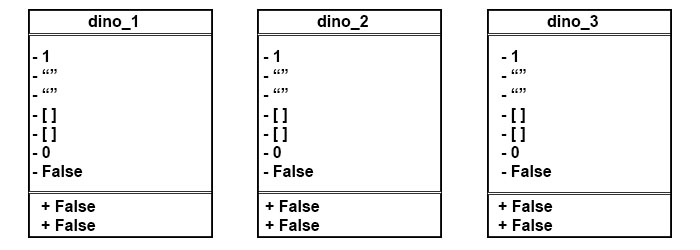
\includegraphics[width=.9\linewidth]{./img/dino_uml_empty.jpg}
\end{center}

Now look those values that has replaced the   tributes. Looks like a big mess. So much so for Object Oriented Programming. This looks like a mockery and a waste of precious time. But its not what it looks like here the attribute values can be over-written for each individual instances.
\begin{verbatim}
dino_1.era = 234
dino_1.name = "Tyranosorus rex"
dino_1.locomotion = "walking"
dino_1.food_habbits = ["dinosaurs", "insects", "fishes"]
dino_1.habitat = ["grasslands"]
dino_1.size = 12
dino_1.flight = False
# We can even use methods
print(dino_1.identifyDinosaur("Tyranosorus rex"))            #Result: True
print(dino_1.checkIfDinosaur())                              #Result: True
\end{verbatim}

Similiarly we can do the same treatment to the instances dino\(_{\text{2}}\) and dino\(_{\text{3}}\).


\begin{verbatim}
dino_2.era = 238.7
dino_2.name = "Mosasaurus"
dino_2.locomotion = "swimming"
dino_2.food_habbits = ["molluscs", "fishes"]
dino_2.habitat = ["seas", "oceans"]
dino_2.size = 17
dino_2.flight = False
dino_3.era = 22
dino_3.name = "Pteranodon"
dino_3.locomotion = "flying"
dino_3.food_habbits = ["insects", "fishes"]
dino_3.habitat = ["mountains", "marshes"]
dino_3.size = 9
dino_3.flight = True
# We can even use methods
print(dino_2.identifyDinosaur("Mosasaurus"))            #Result: True
print(dino_2.checkIfDinosaur())                         #Result: True
print(dino_3.identifyDinosaur("Pteranodon"))            #Result: True
print(dino_3.checkIfDinosaur())                         #Result: False
\end{verbatim}

Hence the representation of these tables have changed,

\begin{center}
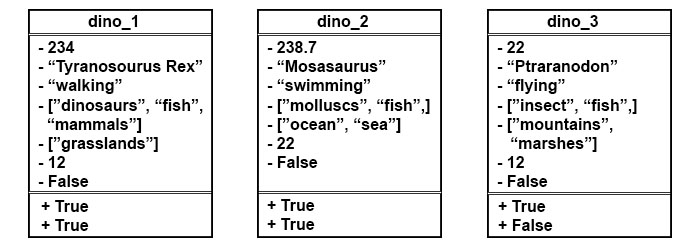
\includegraphics[width=.9\linewidth]{./img/dino_uml.jpg}
\end{center}
The whole process may be given a GUI.

\begin{figure}[htbp]
\centering
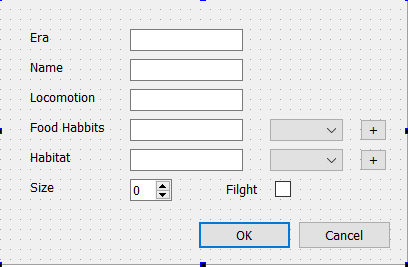
\includegraphics[width=.9\linewidth]{./img/dino_gui.png}
\caption{\label{fig:orgaff86e5}
This is a gui to insert dinosaur information to the computer.}
\end{figure}

Well while creating an instance what if we could place the values of era, name, locomotion, habitat, food\(_{\text{habbits,size}}\) and flight as a parameter it would spare us the extra time in gathering information one by one. One way of doing that is by initializing the instance as,

\begin{verbatim}
dino_1 = Dinosaurs(234, "Tyranosorus rex", "walking", ["dinosaurs", "insects", "fishes"], ["grasslands"], 12, False) 
\end{verbatim}

This way whenever we press ok in the GUI shown in figure1 we end up creating an instace with the initiated values. Constructors are special class members which are called by the Python interpreter every time an object of that class is instantiated. A constructor of a class is actually a member function of the class its declared as: 
\begin{verbatim}
class Cowboys:
    def __init__():
''' This is the constructor '''
        pass
\end{verbatim}
Similiarly like a constructor there is a destrutor. Its use unlike the constructor is to destroy/delete an instance of the class. Its declared as:
\begin{verbatim}
class Cowboys:
    def __init__(self):
    # Used to construct the instance
        pass

    def __del__(self):
    # Used to destroy an instance
        pass
\end{verbatim}

These double underscore also known as dunder methods are also called magic methods. Lets recreate Dinosaurs class using the constructor method.

\begin{verbatim}
class Dinosaurs():
    def __init__(self, era, name, locomotion, habitat, food_habbits, size, flight):
''' This is the constructor '''
        self.era = era
        self.name = name
        self.locomotion = locomotion
        self.habitat = habitat
        self.food_habbits = food_habbits
        self.size = size
        self.flight = flight

    def __del__(self):
        return f'Instance Destroyed with name {self.name}'
\end{verbatim}

So now,
\begin{verbatim}
dino_1 = Dinosaurs(234, "Tyranosorus rex", "walking", ["dinosaurs", "insects", "fishes"], ["grasslands"], 12, False)
dino_2 = Dinosaurs(238.7, "Mosasasaurus", "swimming", ["molluscs", "fish"], ["ocean", "sea"], 22, False)
dino_3 = Dinosaurs(234, "Ptarandon", "flying", ["insect", "fish"], ["mountains", "marshes"], 9, True)

del dino_2    # Deletes/destroys dino_2 instance
\end{verbatim}
\end{document}